% !TEX TS-program = pdflatex
% !TEX encoding = UTF-8 Unicode

\documentclass{beamer}
%\documentclass[handout]{beamer}

%\setbeamertemplate{background canvas}[vertical shading][bottom=white,top=structure.fg!25]
% or whatever

\usetheme[compress]{Amsterdam}
%\setbeamertemplate{headline}{}
%\setbeamertemplate{footline}{}
%\setbeamersize{text margin left=0.5cm}
  
\usepackage[english]{babel}
\usepackage{listings}
\usepackage{geometry}
\usepackage{hyperref}

\usepackage{color}
\usepackage[T1]{fontenc}
\usepackage[utf8]{inputenc}
\usepackage{lmodern}
\usepackage{etoolbox}

\usepackage{tikz}
\usetikzlibrary{shapes,arrows}

\usepackage{multicol}
\lstset{
basicstyle=\scriptsize\ttfamily,
columns=flexible,
breaklines=true,
numbers=left,
%stepsize=1,
numberstyle=\tiny,
backgroundcolor=\color[rgb]{0.85,0.90,1}
}


\begin{document}

\title[Big Data and Automated Content Analysis]{\textbf{A Practical Introduction to Machine Learning in Python} \\Day 2 - Tuesday \\ »Preparing for Analysis: From text to features«}
\author[Damian Trilling, Anne Kroon]{Damian Trilling \\ Anne Kroon \\ ~ \\ \footnotesize{d.c.trilling@uva.nl, @damian0604 \\a.c.kroon@uva.nl, @annekroon} \\}
\date{March 10, 2020}
\institute[Gesis]{Gesis}


\tikzstyle{block} = [rectangle, draw, fill=blue!20, 
text width=5em, text centered, rounded corners, minimum height=4em]
\tikzstyle{line} = [draw]
\tikzstyle{pijltje} = [draw, -latex']
\tikzstyle{cloud} = [draw, ellipse,fill=red!20, node distance=3cm,
minimum height=2em, text width=4em, text centered,]



\setbeamercovered{transparent}

\begin{frame}{}
\titlepage
\end{frame}

\begin{frame}{Today}
\tableofcontents
\end{frame}

\section{Bottom-up and top-down approaches to computer-aided content analysis}

\begin{frame}[plain]
Brief recap: Bottom-up and top-down approaches to computer-aided content analysis
\end{frame}

\begin{frame}[plain]
\makebox[\linewidth]{
	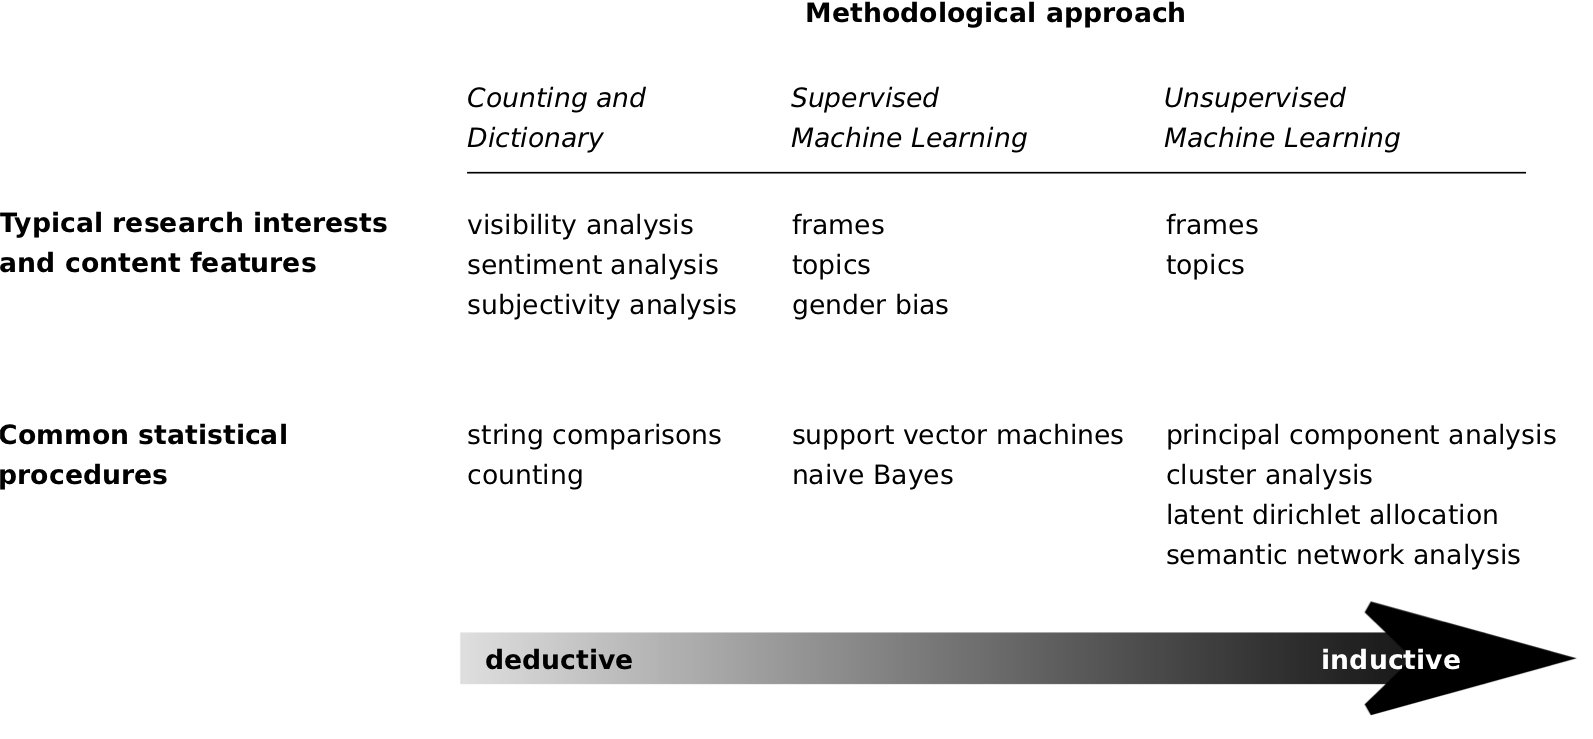
\includegraphics[width=\paperwidth,height=\paperheight,keepaspectratio]{../pictures/boumanstrilling2016_.png}}
\end{frame}


\begin{frame}{Some considerations}
\begin{itemize}[<+->]
	\item Both can have a place in your workflow (e.g., bottom-up as first exploratory step)
	\item You have a clear theoretical expectation? Bottom-up makes little sense.
	\item But in any case: you need to transform your text into something ``countable''.
\end{itemize}
\end{frame}


\section{Bottom-up: Exploratory techniques to explore your data}
\begin{frame}[plain]
Bottom-up: Exploratory techniques to explore your data
\end{frame}
% counter



\begin{frame}{Counting words}
\begin{enumerate}
	\item Split text into words (``tokenization'')
	\item Count words
\end{enumerate}
\end{frame}

\begin{frame}[fragile]{Counting words}
\begin{lstlisting}
from collections import Counter

texts = ['This is the first text text text first', 'And another text yeah yeah']

tokenized_texts = [t.split() for t in texts] 

c = Counter(tokenized_texts[0]) 
print(c.most_common(3) 

c2 = Counter(tokenized_texts[1]) 
print(c2.most_common(3)) 

\end{lstlisting}

\texttt{('text', 3), ('first', 2), ('This', 1)]}

\texttt{[('yeah', 2), ('And', 1), ('another', 1)]}

\pause

\textbf{\textcolor{red}{What do we have to improve?}}

\end{frame}


\begin{frame}[fragile]{Some preprocessing}{(more about this later today)}


lowercasing
\begin{lstlisting}
texts2 = [t.lower() for t in texts]
\end{lstlisting}

removing punctuation (method 1)
\begin{lstlisting}
texts3 = [t.replace('.','').replace(',','').replace('!','') for t in texts]   
\end{lstlisting}

removing punctuation (method 2)
\begin{lstlisting}
import string
trans = str.maketrans('', '', string.punctuation)
texts4 = [t.translate(trans) for t in texts]   
\end{lstlisting}
\end{frame}

\section{Top-down: Regular expressions}
\begin{frame}[plain]
Top-down: Regular expression
\end{frame}



\subsection{What is a regexp?}
\begin{frame}{Regular Expressions: What and why?}
\begin{block}{What is a regexp?}
	\begin{itemize}
		\item<1-> a \emph{very} widespread way to describe patterns in strings
		\item<2-> Think of wildcards like {\tt{*}} or operators like {\tt{OR}}, {\tt{AND}} or {\tt{NOT}} in search strings: a regexp does the same, but is \emph{much} more powerful
		\item<3-> You can use them in many editors (!), in the Terminal, in STATA \ldots and in Python
	\end{itemize}
\end{block}
\end{frame}

\begin{frame}{An example}
\begin{block}{From last week's task}
\begin{itemize}
	\item We wanted to remove everything but words from a tweet
	\item We did so by calling the \texttt{.replace()} method
	\item We could do this with a regular expression as well: \\
	{\tt{ \lbrack \^{}a-zA-Z\rbrack}} would match anything that is not a letter
\end{itemize}
\end{block}
\end{frame}

\begin{frame}{Basic regexp elements}
\begin{block}{Alternatives}
\begin{description}
\item[{\tt{\lbrack TtFf\rbrack}}] matches either T or t or F or f
\item[{\tt{Twitter|Facebook}}] matches either Twitter or Facebook
\item[{\tt{.}}] matches any character
\end{description}
\end{block}
\begin{block}{Repetition}<2->
\begin{description}
\item[{\tt{*}}] the expression before occurs 0 or more times
\item[{\tt{+}}] the expression before occurs 1 or more times
\end{description}
\end{block}
\end{frame}

\begin{frame}{regexp quizz}
\begin{block}{Which words would be matched?}
\tt
\begin{enumerate}
\item<1-> \lbrack Pp\rbrack ython
\item<2-> \lbrack A-Z\rbrack +
\item<3-> RT ?:? @\lbrack a-zA-Z0-9\rbrack *
\end{enumerate}
\end{block}
\end{frame}

\begin{frame}{What else is possible?}
If you google {\tt{regexp}} or {\tt{regular expression}}, you'll get a bunch of useful overviews. The wikipedia page is not too bad, either. 
\end{frame}

\subsection{Using a regexp in Python}
\begin{frame}{How to use regular expressions in Python}
\begin{block}{The module re}
\begin{description}
\item<1->[{\tt{re.findall("\lbrack Tt\rbrack witter|\lbrack Ff\rbrack acebook",testo)}}] returns a list with all occurances of Twitter or Facebook in the string called {\tt{testo}}
\item<1->[{\tt{re.findall("\lbrack 0-9\rbrack +\lbrack a-zA-Z\rbrack +",testo)}}] returns a list with all words that start with one or more numbers followed by one or more letters in the string called {\tt{testo}}
\item<2->[{\tt{re.sub("\lbrack Tt\rbrack witter|\lbrack Ff\rbrack acebook","a social medium",testo)}}] returns a string in which all all occurances of Twitter or Facebook are replaced by "a social medium"
\end{description}
\end{block}
\end{frame}


\begin{frame}[fragile]{How to use regular expressions in Python}
\begin{block}{The module re}
\begin{description}
\item<1->[{\tt{re.match(" +(\lbrack 0-9\rbrack +) of (\lbrack 0-9\rbrack +) points",line)}}] returns  \texttt{None} unless it \emph{exactly} matches the string \texttt{line}. If it does, you can access the part between () with the \texttt{.group()} method.
\end{description}
\end{block}

Example:
\begin{lstlisting}
line="             2 of 25 points"
result=re.match(" +([0-9]+) of ([0-9]+) points",line)
if result:
print ("Your points:",result.group(1))
print ("Maximum points:",result.group(2))
\end{lstlisting}
Your points: 2\\
Maximum points: 25
\end{frame}














\begin{frame}{Possible applications}
\begin{block}{Data preprocessing}
\begin{itemize}
\item Remove unwanted characters, words, \ldots
\item Identify \emph{meaningful} bits of text: usernames, headlines, where an article starts, \ldots
\item filter (distinguish relevant from irrelevant cases)
\end{itemize}
\end{block}
\end{frame}


\begin{frame}{Possible applications}
\begin{block}{Data analysis: Automated coding}
\begin{itemize}
\item Actors
\item Brands
\item links or other markers that follow a regular pattern
\item Numbers (!)
\end{itemize}
\end{block}
\end{frame}

\begin{frame}[fragile,plain]{Example 1: Counting actors}
\begin{lstlisting}
import re, csv
from glob import glob
count1_list=[]
count2_list=[]
filename_list = glob("/home/damian/articles/*.txt")

for fn in filename_list:
  with open(fn) as fi:
    artikel = fi.read()
    artikel = artikel.replace('\n',' ')

    count1 = len(re.findall('Israel.*(minister|politician.*|[Aa]uthorit)',artikel))
    count2 = len(re.findall('[Pp]alest',artikel))

    count1_list.append(count1)
    count2_list.append(count2)

output=zip(filename_list,count1_list, count2_list)
with open("results.csv", mode='w',encoding="utf-8") as fo:
  writer = csv.writer(fo)
  writer.writerows(output)
\end{lstlisting}
\end{frame}




\begin{frame}[fragile]{Example 2: Which number has this Lexis Nexis article?}
\begin{lstlisting}
All Rights Reserved

2 of 200 DOCUMENTS

De Telegraaf

21 maart 2014 vrijdag

Brussel bereikt akkoord  aanpak probleembanken;
ECB krijgt meer in melk te brokkelen

SECTION: Finance; Blz. 24
LENGTH: 660 woorden

BRUSSEL   Europa heeft gisteren op de valreep een akkoord bereikt 
over een saneringsfonds voor banken. Daarmee staat de laatste
\end{lstlisting}

\end{frame}

\begin{frame}[fragile]{Example 2: Check the number of a lexis nexis article}
\begin{lstlisting}
All Rights Reserved

2 of 200 DOCUMENTS

De Telegraaf

21 maart 2014 vrijdag

Brussel bereikt akkoord  aanpak probleembanken;
ECB krijgt meer in melk te brokkelen

SECTION: Finance; Blz. 24
LENGTH: 660 woorden

BRUSSEL   Europa heeft gisteren op de valreep een akkoord bereikt 
over een saneringsfonds voor banken. Daarmee staat de laatste
\end{lstlisting}

\begin{lstlisting}
for line in tekst:
matchObj=re.match(r" +([0-9]+) of ([0-9]+) DOCUMENTS",line)
if matchObj:
numberofarticle= int(matchObj.group(1))
totalnumberofarticles= int(matchObj.group(2))
\end{lstlisting}
\end{frame}


\begin{frame}{Practice yourself!}
\huge{\url{http://www.pyregex.com/}}
\end{frame}

\section{Natural Language Processing}
\begin{frame}
Natural Language Processing
\end{frame}



\begin{frame}{NLP: What and why?}
\begin{block}{What can we do?}
\begin{itemize}
\item<1-> remove stopwords
\item<2-> stemming
\item<3-> parse sentences (advanced)
\end{itemize}
\end{block}
\end{frame}






\subsection{Stopword removal}
\begin{frame}
Natural Language Processing:\\
\textbf{Stopword removal} \\
\vspace{1cm}
\onslide<2>{\emph{Have a look back at last week! The logic of the algorithm is very much related to the one of our first simple sentiment analysis!}}
\end{frame}


\begin{frame}{Stopword removal: What and why?}
\begin{block}{Why remove stopwords?}
\begin{itemize}
\item If we want to identify key terms (e.g., by means of a word count), we are not interested in them
\item If we want to calculate document similarity, it might be inflated
\item If we want to make a word co-occurance graph, irrelevant information will dominate the picture
\end{itemize}
\end{block}
\end{frame}


\begin{frame}[fragile]{Stopword removal: How}
\begin{lstlisting}
testo='He gives her a beer and a cigarette.'
testonuovo=""
mystopwords=['and','the','a','or','he','she','him','her']
for verbo in testo.split():
  if verbo not in mystopwords:
    testonuovo=testonuovo+verbo+" "
\end{lstlisting}
What do we get if we do:
\begin{lstlisting}
print (testonuovo)
\end{lstlisting}
Can you explain the algorithm?
\end{frame}

\begin{frame}[fragile]{We get:}
\begin{lstlisting}
>>> print  (testonuovo)
'He gives beer cigarette. '
\end{lstlisting}
Why is "He" still in there? \\ How can we fix this?
\end{frame}

\begin{frame}[fragile]{Stopword removal}
\begin{lstlisting}
testo='He gives her a beer and a cigarette.'
testonuovo=""
mystopwords=['and','the','a','or','he','she','him','her']
for verbo in testo.split():
  if verbo.lower() not in mystopwords:
    testonuovo=testonuovo+verbo+" "
\end{lstlisting}

\pause

With \textit{list comprehension} and the \texttt{.join()} method, you can achieve the same thing in one line:

\begin{lstlisting}
tn2 = " ".join([w for w in testo.split() if w not in mystopwords])
\end{lstlisting}
\pause
This is more efficient and more ``pythonic'', but may be more difficult to debug (especially if it gets more complicated)

\end{frame}











\section{When, why, and how do we pre-process?}
\begin{frame}[plain]
When, why, and how do we pre-process?
\end{frame}



\section{Natural Language Processing with NLTK and spacy}
\begin{frame}[plain]
Natural Language Processing with NLTK and spacy
\end{frame}
	
	% ngrams
	
	


\subsection{Stemming}
\begin{frame}{NLP: What and why?}
\begin{block}{Why do stemming?}
	\begin{itemize}
		\item Because we do not want to distinguish between smoke, smoked, smoking, \ldots
		\item Typical preprocessing step (like stopword removal)
	\end{itemize}
\end{block}
\end{frame}









\begin{frame}[fragile]{Stemming}
{\footnotesize{(with NLTK, see Bird, S., Loper, E., \& Klein, E. (2009). \emph{Natural language processing with Python}. Sebastopol, CA: O’Reilly.)}}
\begin{lstlisting}
from nltk.stem.snowball import SnowballStemmer
stemmer=SnowballStemmer("english")
frase="I am running while generously greeting my neighbors"
frasenuevo=""
for palabra in frase.split():
  frasenuevo=frasenuevo + stemmer.stem(palabra)  + " "
\end{lstlisting}
If we now did {\tt{print(frasenuevo)}}, it would return:
\begin{lstlisting}
i am run while generous greet my neighbor
\end{lstlisting}
\end{frame}

\begin{frame}[fragile]{Stemming and stopword removal - let's combine them!}
\begin{lstlisting}
from nltk.stem.snowball import SnowballStemmer
from nltk.corpus import stopwords
stemmer=SnowballStemmer("english")
mystopwords = stopwords.words("english")
frase="I am running while generously greeting my neighbors"
frasenuevo=""
for palabra in frase.lower().split():
  if palabra not in mystopwords:
    frasenuevo=frasenuevo + stemmer.stem(palabra)  + " "
\end{lstlisting}
Now, {\tt{print(frasenuevo)}} returns:
\begin{lstlisting}
run generous greet neighbor
\end{lstlisting}
Perfect!

\pause
\small
Or:
\begin{lstlisting}
print(" ".join([stemmer.stem(p) for p in frase.lower().split() if p not in mystopwords]))
\end{lstlisting}


\onslide<3>{
\tiny{In order to use \texttt{nltk.corpus.stopwords}, you have to download that module once. You can do so by typing the following in the Python console and selecting the appropriate package from the menu that pops up: \\ \texttt{import nltk\\nltk.download()}\\NB: Don't download everything, that's several GB.\\}}
\end{frame}

{\setbeamercolor{background canvas}{bg=black}
\begin{frame}[plain]
\makebox[\linewidth]{
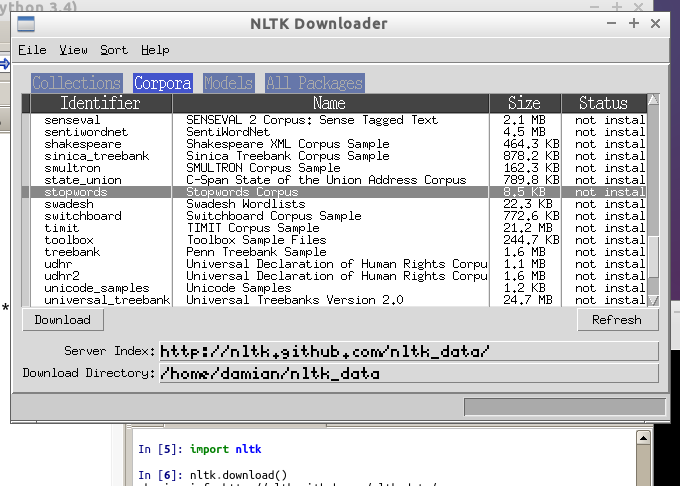
\includegraphics[width=\paperwidth,height=\paperheight,keepaspectratio]{../pictures/nltk-download.png}}
\end{frame}
}


\subsection{ngrams}
Instead of just looking at single words (unigrams), we can also use adjacent words (bigrams).
\begin{frame}[fragile]{ngrams}
\begin{lstlisting}
import nltk
texts = ['This is the first text text text first', 'And another text yeah yeah']
texts_bigrams = [["_".join(tup) for tup in nltk.ngrams(t.split(),2)] for t in texts]
print(texts_bigrams)
\end{lstlisting}
\texttt{[['This\_is',
	'is\_the',
	'the\_first',
	'first\_text',
	'text\_text',
	'text\_text',
	'text\_first'],
	['And\_another', 'another\_text', 'text\_yeah', 'yeah\_yeah']]
}

Typically, we would combine both.
\pause
\textbf{\textcolor{red}{What do you think? Why is this useful? (and what may be drawbacks?)}}
\end{frame}


\subsection{Parsing sentences}
\begin{frame}{NLP: What and why?}
\begin{block}{Why parse sentences?}
\begin{itemize}
\item To find out what grammatical function words have
\item and to get closer to the meaning.
\end{itemize}
\end{block}
\end{frame}

\begin{frame}[fragile]{Parsing a sentence}
\begin{lstlisting}
import nltk
sentence = "At eight o'clock on Thursday morning, Arthur didn't feel very good."
tokens = nltk.word_tokenize(sentence)
print (tokens)
\end{lstlisting}

\texttt{nltk.word\_tokenize(sentence)} is similar to sentence.split(), but compare handling of punctuation and the \texttt{didn't} in the output:
\begin{lstlisting}
['At', 'eight', "o'clock", 'on', 'Thursday', 'morning','Arthur', 'did', "n't", 'feel', 'very', 'good', '.']
\end{lstlisting}
\end{frame}


\begin{frame}[fragile]{Parsing a sentence}
Now, as the next step, you can ``tag'' the tokenized sentence:
\begin{lstlisting}
tagged = nltk.pos_tag(tokens)
print (tagged[0:6])
\end{lstlisting}
gives you the following:
\begin{lstlisting}
[('At', 'IN'), ('eight', 'CD'), ("o'clock", 'JJ'), ('on', 'IN'),
('Thursday', 'NNP'), ('morning', 'NN')]
\end{lstlisting}

\onslide<2->{
And you could get the word type of "morning" with \texttt{tagged[5][1]}!
}

\end{frame}


\begin{frame}{More NLP}
\Huge{Look at \url{http://nltk.org}}

\end{frame}


\begin{frame}{More NLP}
\Huge{Look at \url{http://spacy.io}}
\end{frame}


\begin{frame}[fragile]{Example: Named Entity Recognition with spacy}
Terminal:

\begin{lstlisting}
sudo pip3 install spacy
sudo python3 -m spacy download nl    # or en, de, fr ....
\end{lstlisting}

Python:

\begin{lstlisting}
import spacy
nlp = spacy.load('nl')
doc = nlp('De docent heet Damian, en hij geeft vandaag les. Daarnaast is hij een onderzoeker, net zoals Anne. Ze werken allebei op de UvA')
for ent in doc.ents:
print(ent.text,ent.label_)
\end{lstlisting}

returns:

\begin{lstlisting}
Damian MISC
Anne PER
UvA LOC
\end{lstlisting}  

\end{frame}



\begin{frame}{More NLP}
\Huge{Look at \url{http://nlp.stanford.edu}}
\end{frame}


\begin{frame}{More NLP}
\Huge{Look at \url{https://www.clips.uantwerpen.be/pattern}}
\end{frame}






	
\section{From text to feature: count vectorizers and tf-idf vectorizers}
\begin{frame}[plain]
From text to feature: count vectorizers and tf-idf vectorizers
\end{frame}	



\begin{frame}{What is a vectorizer}
\begin{itemize}[<+->]
	\item Transforms a list of texts into a sparse (!) matrix (of word frequencies)
	\item Vectorizer needs to be ``fitted'' to the training data (learn which words (features) exist in the dataset and assign them to columns in the matrix)
	\item Vectorizer can then be re-used to transform other datasets 
\end{itemize}
\end{frame}


\begin{frame}{Different vectorizers}
\begin{enumerate}[<+->]
	\item CountVectorizer (=simple word counts)
	\item TfidfVectorizer (word counts (``term frequency'') weighted by number of documents in which the word occurs at all (``inverse document frequency''))
\end{enumerate}

\pause
$$tfidf_{t,d} = tf_{t,d} \cdot idf_{t}$$

There are different ways to weigh the idf score. A common one is taking the logarithm:

$$idf_{t} = \log \frac{N}{n_t}$$

where $N$ is the total number of documents and $n_t$ is the number of documents containing term $t$
\end{frame}

\begin{frame}{Different vectorizer options}
\begin{itemize}
\item Preprocessing (e.g., stopword removal)
\item Remove words below a specific threshold (``occurring in less than $n=5$ documents'') $\Rightarrow$ spelling mistakes etc.
\item Remove words above a specific threshold (``occuring in more than 50\% of all documents) $\Rightarrow$ de-facto stopwords
\item Not only to improve prediction, but also performance (can reduce number of features by a huge amount)
\end{itemize}
\end{frame}


\begin{frame}[fragile]{Using a scikit-learn vectorizer}
\begin{lstlisting}
from sklearn.feature_extraction.text import Couectorizer
texts = ['This is the first text text text first', 'And another text yeah yeah']
vec = CountVectorizer(texts)
vec.fit_transform(texts) 

# if we want to see what it looks like
# DON'T DO THIS WITH LARGE MATRICES!
print(vec.get_feature_names())
print(vec.transform(texts).todense()) 
\end{lstlisting}
\end{frame}


\section{Summing up: From text to feature}

\begin{frame}[plain]
Summing up: From text to feature
\end{frame}

\begin{frame}{Before we can do machine learning, we need to make features}

\begin{itemize}[<+->]
	\item typically, (weighted) word frequencies (count vs tf$\cdot$idf)
	\item normalization steps first (lowercasing, punctuation, (stemming/lemmatizing))
	\item potentially also other feature (e.g., named entities -- or only specific word types)
	\item unigrams vs ngrams
	\item pruning (removing extremes)
\end{itemize}


\end{frame}


\end{document}